% Variant B: two histories, one window, one prediction.
% Schematic of a fixed declared scalar input-output map; exact expectations.
\RequirePackage{fix-cm}
\documentclass[10pt]{article}
\usepackage[paperwidth=17.9197cm,paperheight=17.9197cm,margin=0pt]{geometry}
\usepackage[T1]{fontenc}
\usepackage{helvet}
\usepackage{amsmath,amssymb}
\usepackage{tikz}
\usetikzlibrary{arrows.meta,calc,decorations.pathreplacing}
\renewcommand{\familydefault}{\sfdefault}
\pagestyle{empty}
\setlength{\parindent}{0pt}
\pdfinfoomitdate=1
\pdftrailerid{}
\pdfsuppressptexinfo=15
\definecolor{ink}{HTML}{202A35}
\definecolor{muted}{HTML}{697887}
\definecolor{blue}{HTML}{2769B0}
\definecolor{teal}{HTML}{138A83}
\definecolor{orange}{HTML}{D57525}
\definecolor{rule}{HTML}{DDE4EB}
\tikzset{
  every node/.style={font=\fontsize{10.5}{12.3}\selectfont,text=ink,inner sep=1pt},
  arrow/.style={-{Stealth[length=2.0mm,width=1.55mm]},line width=.65pt,draw=muted},
  faint/.style={line width=.6pt,draw=rule},
  wire/.style={line width=.65pt,draw=ink!65},
  letter/.style={font=\bfseries\fontsize{11}{12}\selectfont,anchor=west},
  small/.style={font=\fontsize{9.5}{11.3}\selectfont},
  gate/.style={draw=teal!75,line width=.65pt,rounded corners=1.6pt,fill=teal!5,minimum width=.62cm,minimum height=.58cm},
  measure/.style={draw=ink!65,line width=.65pt,rounded corners=1.6pt,fill=white,minimum width=.47cm,minimum height=.45cm}
}
\newcommand{\network}[3]{%
  \begin{scope}[shift={(#1,#2)}]
    \fill[#3!5] (-.66,-.49) -- (-.16,-.78) -- (.72,-.33) -- (.45,.48) -- (-.52,.44) -- cycle;
    \foreach \a/\b/\c/\d in {-.49/.27/.37/.33,-.49/.27/-.29/-.32,-.49/.27/.08/-.05,.37/.33/.08/-.05,.37/.33/.55/-.27,-.29/-.32/.08/-.05,-.29/-.32/.55/-.27,.08/-.05/.55/-.27}{
      \draw[line width=.65pt,#3!55] (\a,\b)--(\c,\d);
    }
    \foreach \x/\y in {-.49/.27,.37/.33,-.29/-.32,.08/-.05,.55/-.27}{
      \filldraw[fill=white,draw=#3,line width=.8pt] (\x,\y) circle (.074);
    }
    \fill[#3] (.08,-.05) circle (.074);
  \end{scope}%
}
\begin{document}
\noindent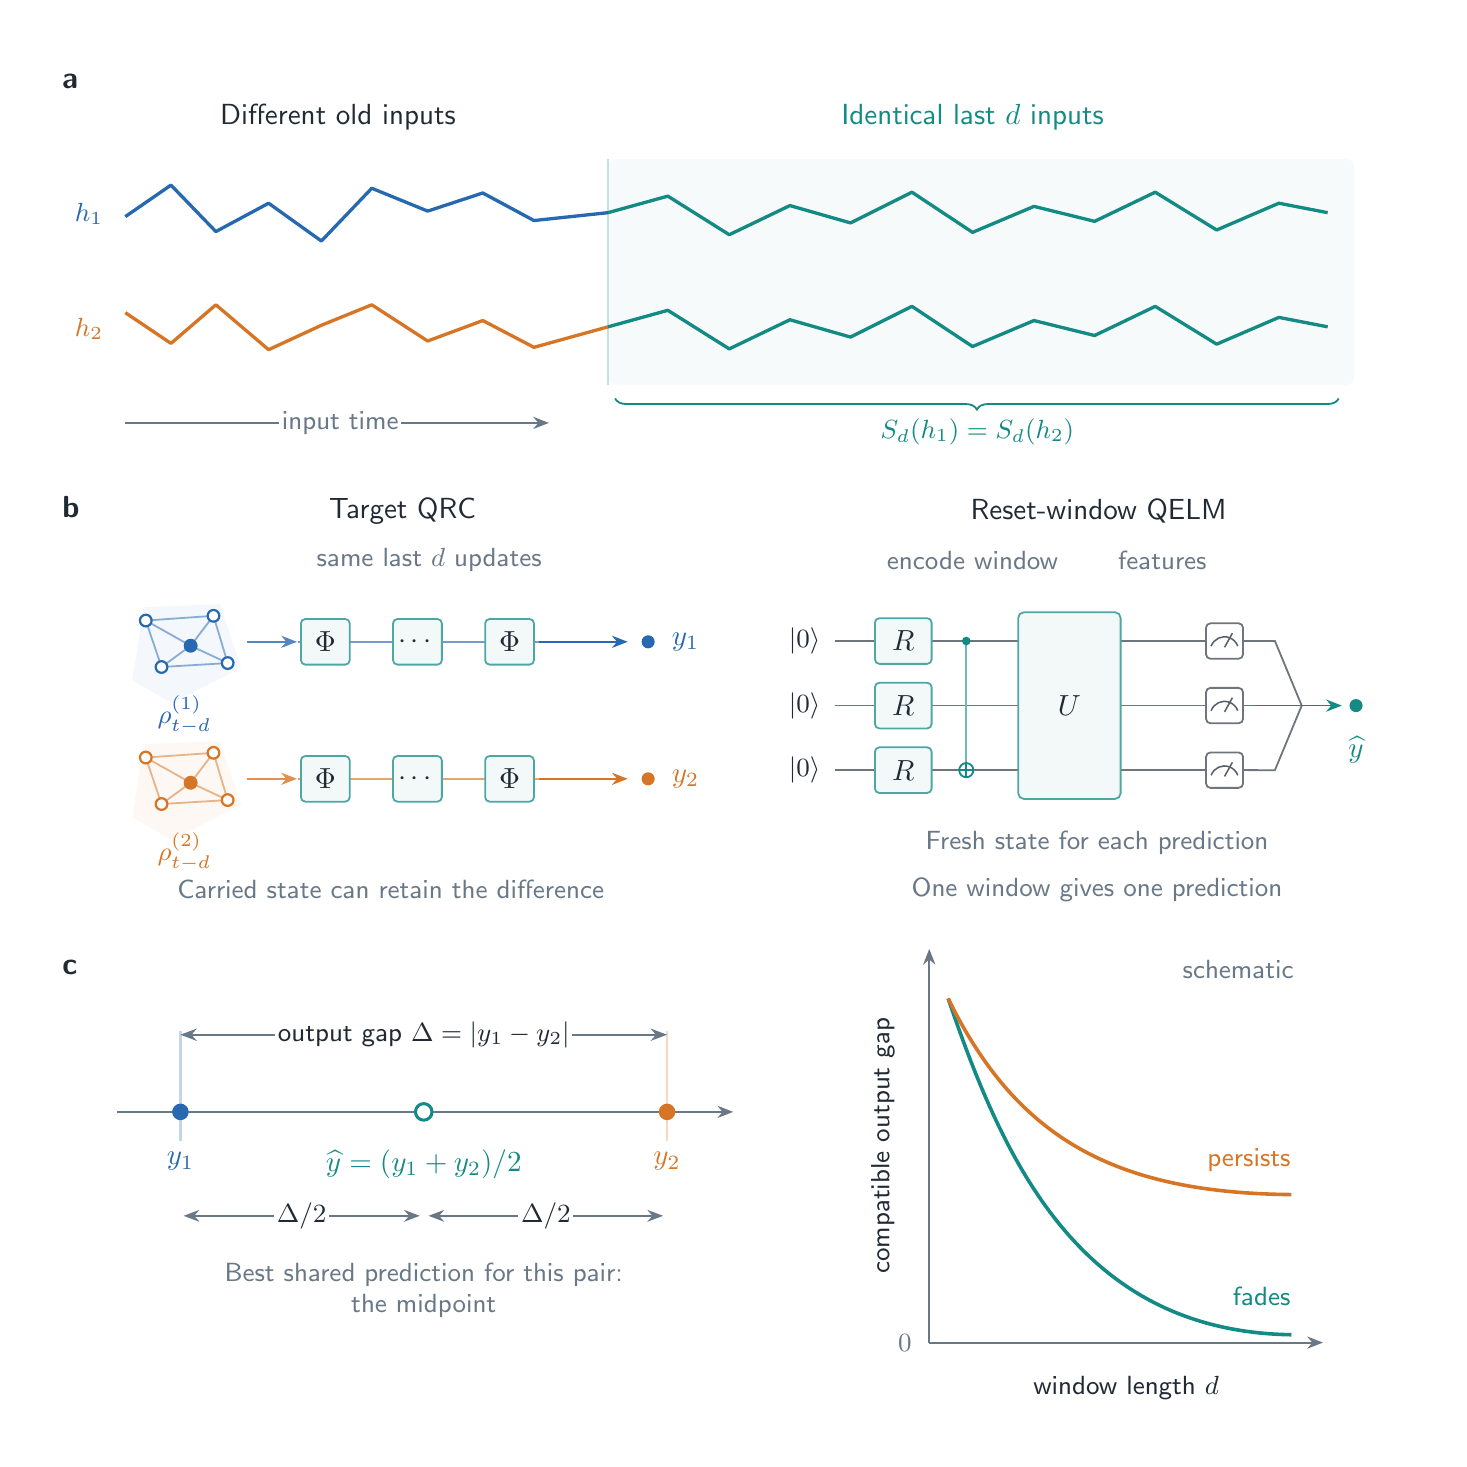
\begin{tikzpicture}[x=1cm,y=1cm]
\path[use as bounding box] (0,0) rectangle (17.9197,17.9197);
\clip (0,0) rectangle (17.9197,17.9197);

% a: the information presented to the two models.
\node[letter] at (.40,17.23) {a};
\node at (3.94,16.78) {Different old inputs};
\node[text=teal] at (12.00,16.78) {Identical last $d$ inputs};
\fill[teal!4,rounded corners=3pt] (7.37,13.38) rectangle (16.85,16.25);
\draw[teal!26,line width=.65pt] (7.37,13.38)--(7.37,16.25);
\node[small,text=blue,anchor=east] at (1.00,15.55) {$h_1$};
\node[small,text=orange,anchor=east] at (1.00,14.10) {$h_2$};
\draw[line width=1.2pt,blue,line join=round] (1.24,15.52)--(1.82,15.92)--(2.39,15.33)--(3.06,15.69)--(3.73,15.21)--(4.37,15.88)--(5.08,15.59)--(5.78,15.82)--(6.43,15.47)--(7.37,15.57);
\draw[line width=1.2pt,orange,line join=round] (1.24,14.30)--(1.82,13.91)--(2.39,14.40)--(3.06,13.83)--(3.73,14.14)--(4.37,14.40)--(5.08,13.94)--(5.78,14.20)--(6.43,13.86)--(7.37,14.12);
\foreach \y in {15.57,14.12}{
  \draw[line width=1.2pt,teal,line join=round] (7.37,\y)--(8.13,\y+.21)--(8.91,\y-.28)--(9.68,\y+.09)--(10.45,\y-.13)--(11.23,\y+.26)--(12.00,\y-.25)--(12.78,\y+.08)--(13.55,\y-.11)--(14.32,\y+.26)--(15.10,\y-.22)--(15.89,\y+.12)--(16.51,\y);
}
\draw[decorate,decoration={brace,mirror,amplitude=4pt},teal,line width=.65pt] (7.46,13.21)--(16.65,13.21);
\node[small,text=teal] at (12.06,12.78) {$S_d(h_1)=S_d(h_2)$};
\draw[arrow] (1.24,12.90)--(6.62,12.90);
\node[small,fill=white,text=muted] at (3.97,12.90) {input time};

% b: a carried quantum state versus a fresh window encoding.
\node[letter] at (.40,11.83) {b};
\node at (4.76,11.78) {Target QRC};
\node at (13.60,11.78) {Reset-window QELM};
\node[small,text=muted] at (5.10,11.16) {same last $d$ updates};
\node[small,text=muted] at (12.00,11.16) {encode window};
\node[small,text=muted] at (14.41,11.16) {features};

\foreach \y/\col/\idx in {10.12/blue/1,8.38/orange/2}{
  \network{1.99}{\y}{\col}
  \node[small,text=\col] at (1.99,\y-.93) {$\rho^{(\idx)}_{t-d}$};
  \draw[arrow,draw=\col!80] (2.78,\y)--(3.42,\y);
  \draw[wire,draw=\col!65] (3.43,\y)--(6.92,\y);
  \node[gate] at (3.78,\y) {$\Phi$};
  \node[gate] at (4.95,\y) {$\cdots$};
  \node[gate] at (6.12,\y) {$\Phi$};
  \draw[arrow,draw=\col] (6.50,\y)--(7.62,\y);
  \fill[\col] (7.88,\y) circle (.083);
  \node[text=\col,anchor=west] at (8.14,\y) {$y_{\idx}$};
}
\node[small,text=muted] at (4.61,6.97) {Carried state can retain the difference};

\foreach \y in {10.13,9.31,8.49}{
  \node[small,anchor=east] at (10.11,\y) {$|0\rangle$};
  \draw[wire] (10.25,\y)--(15.63,\y);
  \node[gate,minimum width=.72cm] at (11.12,\y) {$R$};
  \node[measure] at (15.20,\y) {};
  \draw[line width=.55pt,draw=ink!75] (15.03,\y-.065) arc[start angle=160,end angle=20,radius=.18];
  \draw[line width=.55pt,draw=ink!75] (15.20,\y-.08)--(15.30,\y+.10);
}
\node[draw=teal!75,line width=.65pt,fill=teal!5,rounded corners=2pt,minimum width=1.30cm,minimum height=2.37cm] at (13.23,9.31) {$U$};
\draw[teal!60,line width=.65pt] (11.92,10.13)--(11.92,8.49);
\fill[teal] (11.92,10.13) circle (.055);
\fill[white] (11.92,8.49) circle (.09);
\draw[teal,line width=.65pt] (11.92,8.49) circle (.09);
\draw[teal,line width=.65pt] (11.92,8.39)--(11.92,8.59);
\draw[teal,line width=.65pt] (11.82,8.49)--(12.02,8.49);
\draw[wire] (15.49,10.13)--(15.84,10.13)--(16.18,9.31);
\draw[wire] (15.49,8.49)--(15.84,8.49)--(16.18,9.31);
\draw[arrow,draw=teal] (15.57,9.31)--(16.69,9.31);
\fill[teal] (16.87,9.31) circle (.083);
\node[text=teal] at (16.87,8.75) {$\widehat y$};
\node[small,text=muted] at (13.58,7.56) {Fresh state for each prediction};
\node[small,text=muted] at (13.58,6.97) {One window gives one prediction};

% c: the scalar collision bound and two possible large-window limits.
\node[letter] at (.40,5.98) {c};
\draw[line width=.8pt,draw=blue!28] (1.94,3.78)--(1.94,5.18);
\draw[line width=.8pt,draw=orange!28] (8.12,3.78)--(8.12,5.18);
\draw[<->,>=Stealth,line width=.65pt,draw=muted] (1.94,5.13)--(8.12,5.13);
\node[fill=white,small] at (5.03,5.13) {output gap $\Delta=|y_1-y_2|$};
\draw[arrow] (1.13,4.15)--(8.96,4.15);
\fill[blue] (1.94,4.15) circle (.105);
\fill[orange] (8.12,4.15) circle (.105);
\filldraw[fill=white,draw=teal,line width=1.1pt] (5.03,4.15) circle (.105);
\node[text=blue] at (1.94,3.52) {$y_1$};
\node[text=orange] at (8.12,3.52) {$y_2$};
\node[text=teal] at (5.03,3.49) {$\widehat y=(y_1+y_2)/2$};
\draw[<->,>=Stealth,line width=.6pt,draw=muted] (1.98,2.83)--(4.98,2.83);
\draw[<->,>=Stealth,line width=.6pt,draw=muted] (5.09,2.83)--(8.07,2.83);
\node[small,fill=white] at (3.48,2.83) {$\Delta/2$};
\node[small,fill=white] at (6.58,2.83) {$\Delta/2$};
\node[small,align=center,text=muted] at (5.03,1.88) {Best shared prediction for this pair:\\the midpoint};

% Square 5 x 5 cm axes; the curves are schematic, not simulation data.
\draw[arrow] (11.45,1.22)--(16.45,1.22);
\draw[arrow] (11.45,1.22)--(11.45,6.22);
\node[small,rotate=90] at (10.86,3.72) {compatible output gap};
\node[small] at (13.95,.64) {window length $d$};
\node[small,text=muted,anchor=east] at (11.27,1.22) {$0$};
\draw[teal,line width=1.3pt] (11.69,5.59) .. controls (12.40,3.51) and (13.37,1.36) .. (16.05,1.32);
\draw[orange,line width=1.3pt] (11.69,5.59) .. controls (12.53,3.88) and (13.72,3.12) .. (16.05,3.10);
\node[small,text=orange,anchor=south east] at (16.08,3.35) {persists};
\node[small,text=teal,anchor=south east] at (16.08,1.65) {fades};
\node[small,text=muted,anchor=east] at (16.12,5.96) {schematic};
\end{tikzpicture}
\end{document}
